\documentclass[tikz,border=10pt]{standalone}
\usepackage{tikz}
\usetikzlibrary{shapes,arrows,positioning,fit,backgrounds}

\begin{document}
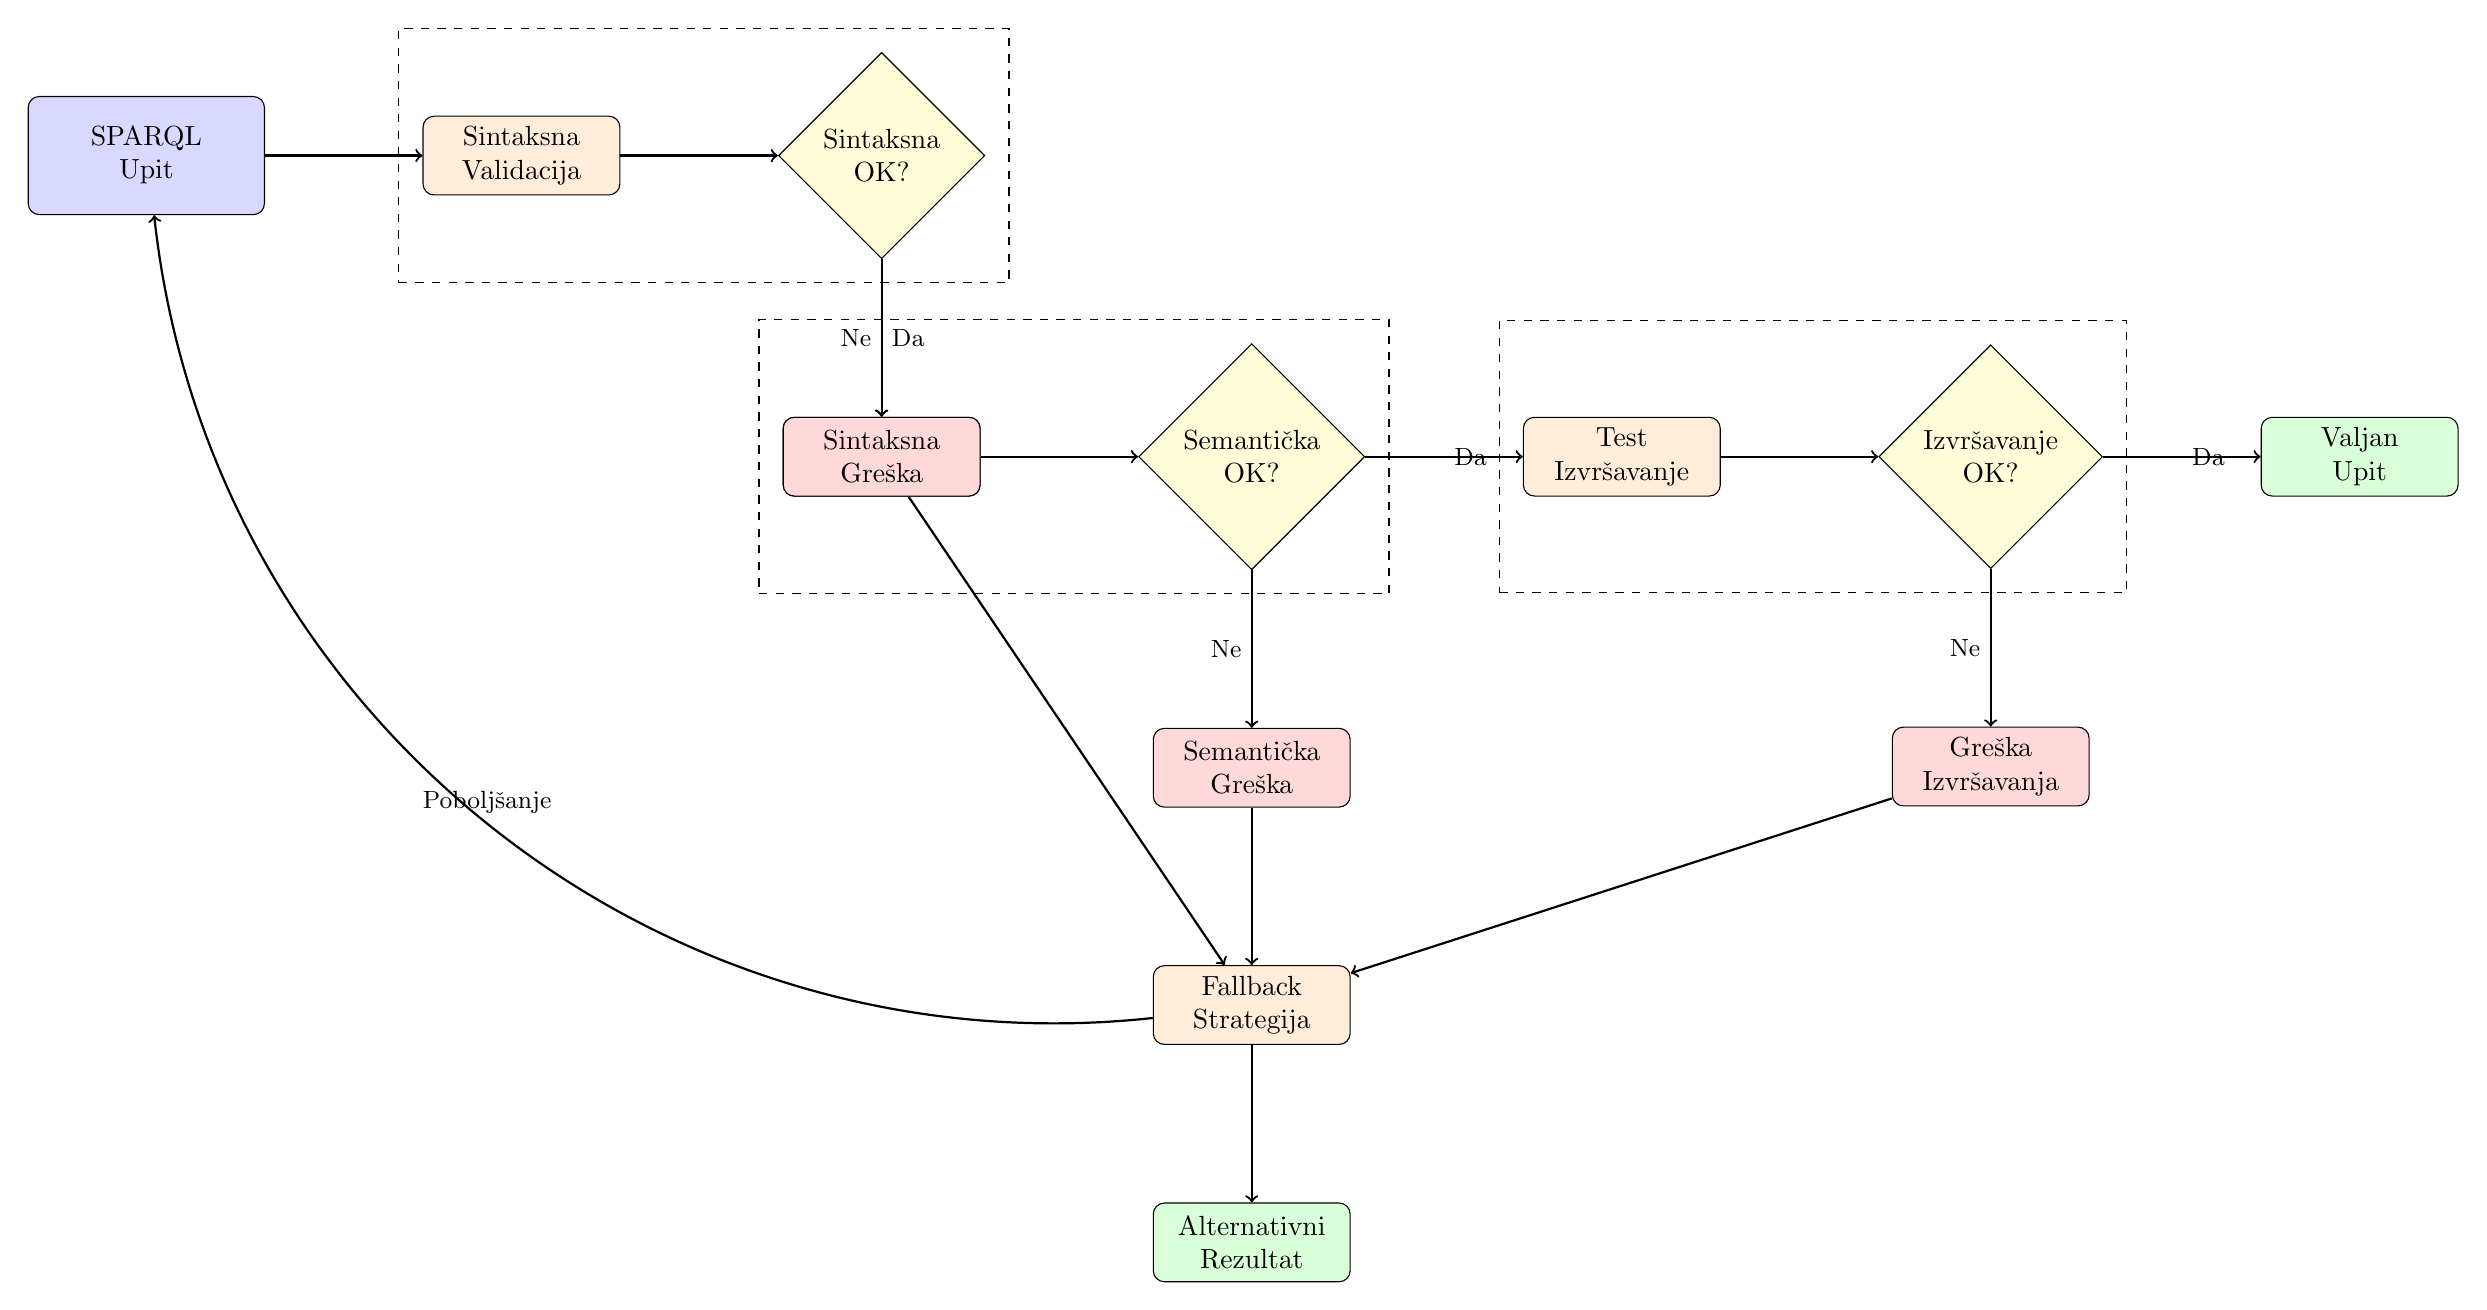
\begin{tikzpicture}[
    node distance=2cm,
    input/.style={rectangle, draw, rounded corners, minimum width=3cm, minimum height=1.5cm, align=center, fill=blue!15},
    process/.style={rectangle, draw, rounded corners, minimum width=2.5cm, minimum height=1cm, align=center, fill=orange!15},
    decision/.style={diamond, draw, minimum width=2cm, minimum height=1.5cm, align=center, fill=yellow!15},
    output/.style={rectangle, draw, rounded corners, minimum width=2.5cm, minimum height=1cm, align=center, fill=green!15},
    error/.style={rectangle, draw, rounded corners, minimum width=2.5cm, minimum height=1cm, align=center, fill=red!15},
    arrow/.style={->, thick},
    label/.style={font=\small}
]

% Input
\node[input] (sparql) {SPARQL\\Upit};

% Validation steps
\node[process, right=of sparql] (syntax) {Sintaksna\\Validacija};
\node[decision, right=of syntax] (syntax_ok) {Sintaksna\\OK?};

% Semantic validation
\node[process, below=of syntax_ok] (semantic) {Semantička\\Validacija};
\node[decision, right=of semantic] (semantic_ok) {Semantička\\OK?};

% Execution
\node[process, right=of semantic_ok] (execute) {Test\\Izvršavanje};
\node[decision, right=of execute] (execute_ok) {Izvršavanje\\OK?};

% Success path
\node[output, right=of execute_ok] (success) {Valjan\\Upit};

% Error handling
\node[error, below=of syntax_ok] (syntax_error) {Sintaksna\\Greška};
\node[error, below=of semantic_ok] (semantic_error) {Semantička\\Greška};
\node[error, below=of execute_ok] (execution_error) {Greška\\Izvršavanja};

% Error recovery
\node[process, below=2cm of semantic_error] (recovery) {Fallback\\Strategija};
\node[output, below=of recovery] (fallback_result) {Alternativni\\Rezultat};

% Background grouping
\begin{scope}[on background layer]
    \node[fit=(syntax)(syntax_ok), draw, dashed, inner sep=0.3cm, label=above:1. Sintaksna Provjera] {};
    \node[fit=(semantic)(semantic_ok), draw, dashed, inner sep=0.3cm, label=above:2. Semantička Provjera] {};
    \node[fit=(execute)(execute_ok), draw, dashed, inner sep=0.3cm, label=above:3. Test Izvršavanja] {};
\end{scope}

% Main flow arrows
\draw[arrow] (sparql) -- (syntax);
\draw[arrow] (syntax) -- (syntax_ok);
\draw[arrow] (syntax_ok) -- node[label, right] {Da} (semantic);
\draw[arrow] (semantic) -- (semantic_ok);
\draw[arrow] (semantic_ok) -- node[label, right] {Da} (execute);
\draw[arrow] (execute) -- (execute_ok);
\draw[arrow] (execute_ok) -- node[label, right] {Da} (success);

% Error paths
\draw[arrow] (syntax_ok) -- node[label, left] {Ne} (syntax_error);
\draw[arrow] (semantic_ok) -- node[label, left] {Ne} (semantic_error);
\draw[arrow] (execute_ok) -- node[label, left] {Ne} (execution_error);

% Error recovery
\draw[arrow] (syntax_error) -- (recovery);
\draw[arrow] (semantic_error) -- (recovery);
\draw[arrow] (execution_error) -- (recovery);
\draw[arrow] (recovery) -- (fallback_result);

% Feedback loop
\draw[arrow, bend left=45] (recovery) to node[label, above] {Poboljšanje} (sparql);

\end{tikzpicture}
\end{document} 